\documentclass{article}
\usepackage[english]{babel}
\usepackage[utf8]{inputenc}
\usepackage{amsmath}
\usepackage{amssymb}
\usepackage{minted}
\usepackage{listings}
\usepackage{xcolor}
\usepackage{graphicx}
\usepackage{pgf}
\usepackage{algorithm}% http://ctan.org/pkg/algorithms
\usepackage{algorithmicx}
\usepackage{algpseudocode}% http://ctan.org/pkg/algorithmicx
% \usepackage{tikz-cd}
\usepackage{tikz}
\usetikzlibrary{arrows.meta, positioning}
\usepackage{comment}
\usepackage{float}
\usepackage{circuitikz}
\usepackage{import}
\usepackage{xifthen}
\usepackage{pdfpages}
\usepackage{pgfplots}
\pgfplotsset{compat=1.18}
\usepackage{pgfplotstable}
\usepackage{transparent}
\usepackage{listings}
\setlength{\parskip}{1em} 

\newcommand{\incfig}[1]{%
    \def\svgwidth{\columnwidth}
    \import{./figures/}{#1.pdf_tex}
}

\newtheorem{remark}{Remark}
\newtheorem{definition}{Definition}
\newtheorem{property}{Property}

\setlength\parindent{0pt}

\newcommand{\pder}[2]{\frac{\partial #1}{\partial #2}}

\title{Decentralized Grid Control in COLMENA \\ Activity 3}
\author{Pablo de Juan Vela $^{1}$, Marco Muttoni $^{1}$, Josep Fanals i Batllori $^{1}$ \\
        \small $^{1}$eRoots Analytics, Barcelona, Spain \\
}
\date{\today}

\usepackage[style=ieee]{biblatex}
\addbibresource{ref.bib}

\begin{document}
\maketitle
\section{Introduction}

In this phase, we present the evaluation of the prototype developed to enable distributed control of electrical grids through autonomous agents. Building on the prototype, we scaled the existing tests and deployed the control scheme in the NPCC grid \cite{grids:npcc} to assess its behaviour under a wide range of conventional and abnormal operating scenarios. We also test different communication schemes between the agents and the interaction with previous roles.

The evaluation focuses on examining the viability of the system’s response in terms of several key performance indicators (KPIs), such as grid robustness, voltage ranges, branch overloads, short-circuit currents, and response times. These KPIs will be measured and analysed across different configurations of the initial system, aiming to demonstrate the platform’s ability to adapt and reconfigure effectively in dynamic conditions.

\section{Evaluation criteria}

In this section we present different criteria and modifications to the initial prototype so that we can compare the changes and how well does COLMENA adapt to these modifications.

\subsection{Agent Coordination Schemes}

One key aspect of the MPC implementation in COLMENA is how the different agents share data between each other. On our previous work, the different agents were completely decentralized: each agent sent the data relative to their primal variables through a predefined channel to only one other agent. This scheme is represented in \ref{fig:distributed_scheme}. 

In the context of COLMENA, we implemented a different scheme in which an asynchronously activated coordinator role receives the data from the agents through a dedicated communication channel and then saves it in a centralized \texttt{@Data} channel. The  different agents can access the shared data through the centralized channel \ref{fig:centralized_scheme}. We will compare the different KPIs for each scenario.

\begin{figure}[ht]
\centering
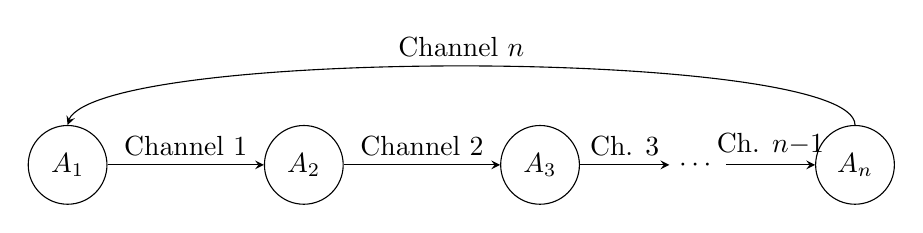
\begin{tikzpicture}[>=stealth, node distance=3cm]

% Define agents
\node[circle, draw, minimum size=1cm] (A1) {$A_1$};
\node[circle, draw, minimum size=1cm, right of=A1] (A2) {$A_2$};
\node[circle, draw, minimum size=1cm, right of=A2] (A3) {$A_3$};
\node (dots) [right of=A3, node distance=2cm] {$\cdots$};
\node[circle, draw, minimum size=1cm, right of=dots, node distance=2cm] (An) {$A_n$};

% Arrows with channel names
\draw[->] (A1) -- (A2) node[midway, above] {Channel 1};
\draw[->] (A2) -- (A3) node[midway, above] {Channel 2};
\draw[->] (A3) -- (dots) node[midway, above] {Ch. 3};
\draw[->] (dots) -- (An) node[midway, above] {Ch. $n{-}1$};

% Last arrow: from top of An to top of A1
\path (An.north) ++(0,1) coordinate (control1);
\path (A1.north) ++(0,1) coordinate (control2);
\draw[->] (An.north) .. controls (control1) and (control2) .. (A1.north)
  node[midway, above, sloped] {Channel $n$};

\end{tikzpicture}
\caption{Data flow among agents in MPC implementation.}
\label{fig:distributed_scheme}
\end{figure}

\begin{figure}[ht]
\centering
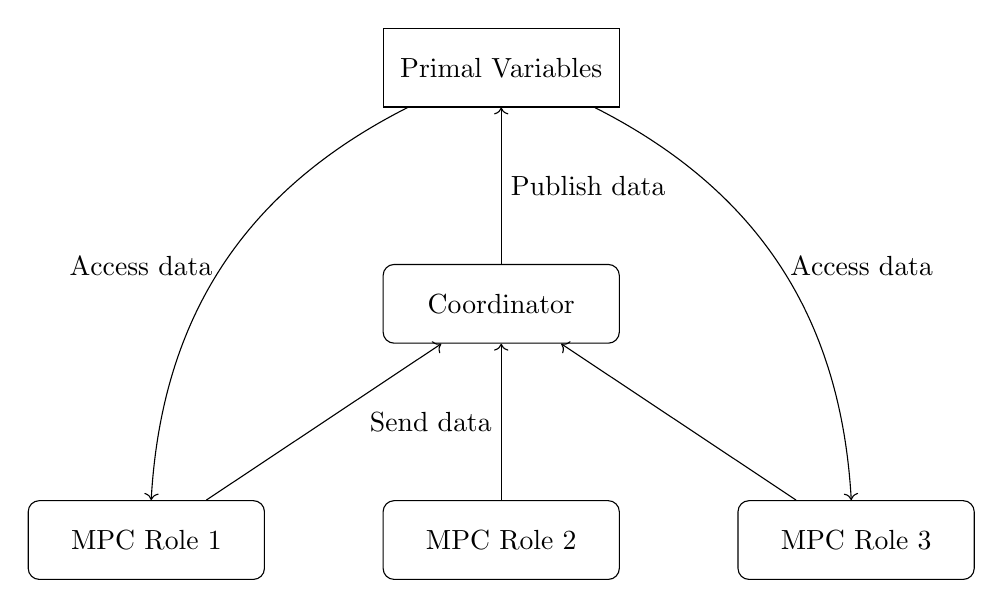
\begin{tikzpicture}[node distance=3cm, auto]

% Define styles for the nodes
\tikzstyle{role} = [rectangle, rounded corners, draw=black, fill=white, minimum height=1cm, minimum width=3cm, text centered]
\tikzstyle{data} = [rectangle, draw=black, fill=white, minimum height=1cm, minimum width=3cm, text centered]

% Nodes
\node (primal) [data] {Primal Variables};
\node (coordinator) [role, below of=primal] {Coordinator};
\node (mpc1) [role, below of=coordinator, left=3cm] {MPC Role 1};
\node (mpc2) [role, below of=coordinator] {MPC Role 2};
\node (mpc3) [role, below of=coordinator, right=3cm] {MPC Role 3};

% Arrows
\draw[->] (coordinator) -- (primal) node[midway, right] {Publish data};
\draw[->, bend right=30] (primal) to node[midway, left] {Access data} (mpc1);
\draw[->, bend left=30] (primal) to node[midway, right] {Access data} (mpc3);
\draw[->] (mpc1) -- (coordinator) node[midway, left] {};
\draw[->] (mpc2) -- (coordinator) node[midway, left] {Send data};
\draw[->] (mpc3) -- (coordinator) node[midway, right] {};

\end{tikzpicture}
\caption{Data flow among roles in the centralized MPC implementation.}
\label{fig:centralized_scheme}
\end{figure}


\subsection{Scalability}

\subsubsection*{Grid Scalability}

The NPCC (Northeastern Power Coordinating Council) grid is an interconnected power system that serves the northeastern United States and parts of Canada. The NPCC 140-Bus system grid model\cite{grids:npcc} is a reduced model of the real life NPCC grid. It consists of 6 different areas, 140 buses, and 46 synchronous generators \ref{fig:npcc}. Given its size and complexity, the NPCC grid requires advanced coordination to ensure reliable operation, particularly in managing power flows, voltage stability, and grid frequency across large distances.

Scaling the prototype to a grid with more areas is crucial for testing its behavior in more realistic and complex conditions. In a real-world system like the NPCC, multiple control areas need to coordinate effectively to maintain overall system stability. By expanding the prototype, we can simulate how decentralized agents (as in COLMENA) interact and control different parts of the grid. This allows for testing the system's ability to handle dynamic conditions such as faults, and varying energy sources across multiple regions. In the following test, we will deploy COLMENA agents that will respond to perturbations in the grid and compare the evolution of different KPIs (computational power, frequency response...).

\begin{figure}[ht]
\centering
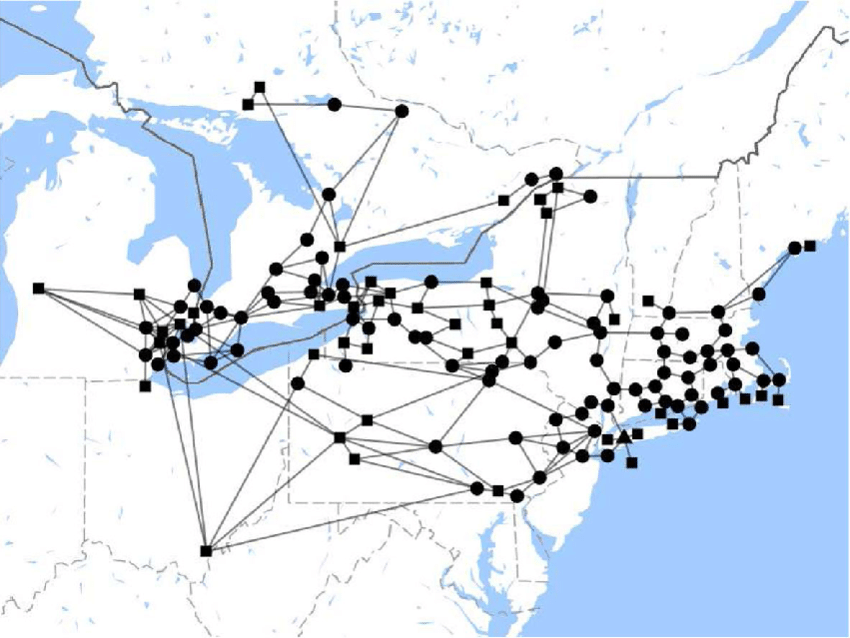
\includegraphics[width=0.8\textwidth]{figures/npcc_grid.png}  % Ensure the path and size are correct
\caption{NPCC grid over a map \cite{grids:npcc}.}
\label{fig:npcc}
\end{figure}

\subsection*{Role \& Agent Scalability}

Another aspect that we want to scale is the number of roles and agents present in the simulation. That's why we also deploy previously explained roles to the simulation. These roles don't manage specific areas but operate locally in specific devices to perform tasks such as adapting the output power of a generator or changing the operation of a converter from Grid Forming (GFM) to Grid Following (GFL). We will study how adding these roles affects the different KPIs and specifically the frequency response. Additionally, we also add converters to the NPCC grid that support the deployment of some of these roles, further making the grid more heterogeneous. The goal of this is to show that all these different roles will work dynamically to maintain the KPIs in an admissible range.

\begin{table}[h]
    \centering
    \small % Reduce font size
    \renewcommand{\arraystretch}{1.2} % Adjust row spacing
    \begin{tabular}{|p{2cm}|p{3cm}|p{3cm}|p{2cm}|} % Adjusted column widths
    \hline
    \textbf{Role} & \textbf{Requirement} & \textbf{Behavior} & \textbf{KPI Trigger} \\
    \hline
    Monitoring & Generator or Converter & Monitors coupled device data & Always Active (Mock KPI) \\
    Automatic Generation Control (AGC) & Generator or Converter Compatible & Activates automatic secondary frequency response & $\omega \notin [\omega_{\min},  \omega_{\max}]$\\
    GFM Activation & Converter Compatible & Switches converter mode from GFL to GFM & $\omega \notin [\omega_{\min},  \omega_{\max}]$\\
    \hline
    \end{tabular}
    \caption{Summary of Roles, Requirements, Behaviors, and Activation KPIs.}
    \label{tab:roles}
\end{table}

\section{Testing}

\subsection*{Test 1: Grid Scalability}

In this test, we compare how the MPC deployment responds to control changes when deployed in a larger grid (NPCC). We start the simulation from a steady state situation, and we disconnect different 5 loads at $t=5$s.We chose the number of loads to be disconnected so that the perturbation is big enough even if the grid is overall larger. This loss of loads results in an increase in frequency to 1.008 p.u . We deploy one agent per area using the \texttt{eager} policy. We observe that the MPC agents are able to adapt the grid to this perturbation in a similar way that in previous tests done in smaller grids \ref{fig:test1}. 

\begin{figure}[ht]
\centering
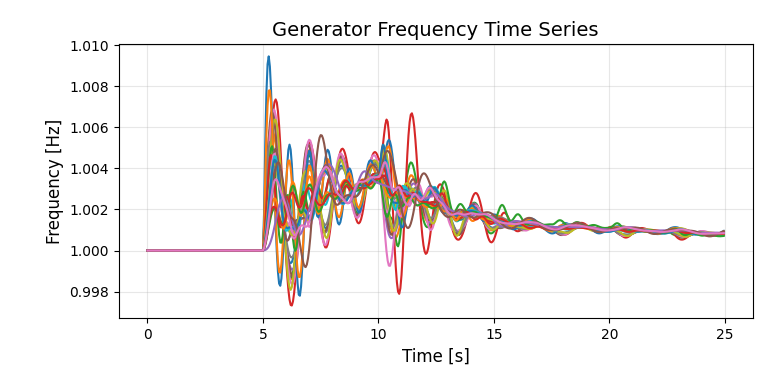
\includegraphics[width=0.8\textwidth]{figures/freq_npcc.png} % Replace with your actual image file path
\caption{Frequency response in the NPCC grid with MPC control}
\label{fig:test1}
\end{figure}

\begin{figure}[ht]
\centering
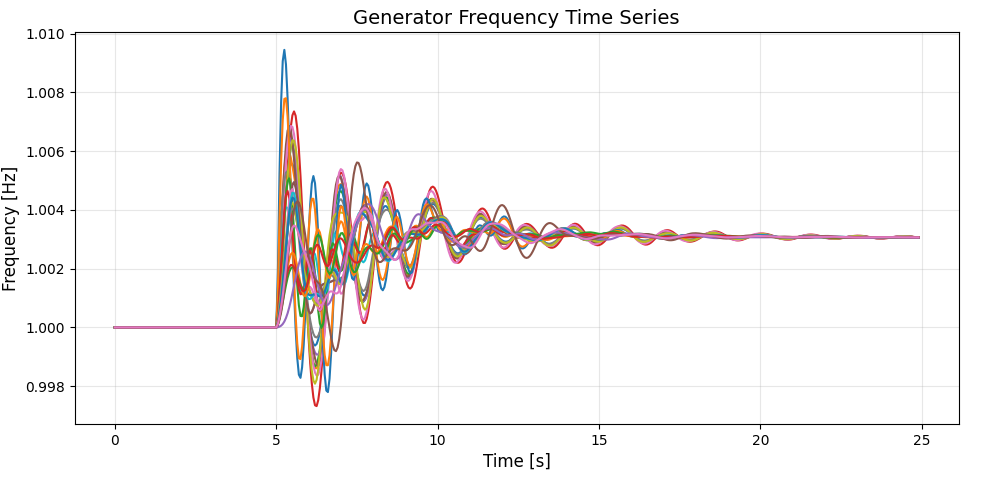
\includegraphics[width=0.8\textwidth]{figures/mpcless_npcc.png} % Replace with your actual image file path
\caption{Frequency response in the NPCC grid without MPC control}
\label{fig:test1less}
\end{figure}


\subsection*{Test 2: Agent Communication Scalability}

In this section we compare the different communications schemes we tried in COLMENA. We perform the same test but as before but changing the scheme that uses a coordinator role. To run this test you just need to change the change the \texttt{script\_name} variable when calling the script \texttt{colmena\_mpc.py} and call it adding \texttt{script\_name = mpc\_with\_coordinator\_role}. The generator's frequency time series results are pretty much identical, meaning in both cases the MPC agents reached the optimal point. However, it can also be interesting to analyze the difference in the use of computational ressources. For this we measure during the testing the time it takes every agent to run an iteration of the MPC role and we separate between communication time that is the time that is closely related to the COLMENA tools and the rest that is more correlated with the MPC itself. For this we compare the time spent in the previous setup with a different setups for the centralized approach.  

\begin{itemize}
\item NPCC :we deploy 8 agents in total, 6 agents for the area control and 2 agents exclusively for running the coordinator role.
\item IEEE39 :we deploy 3 agents in total, 2 agents for the area control and 1 agents exclusively for running the coordinator role.
\end{itemize}

\begin{figure}[ht]
\centering
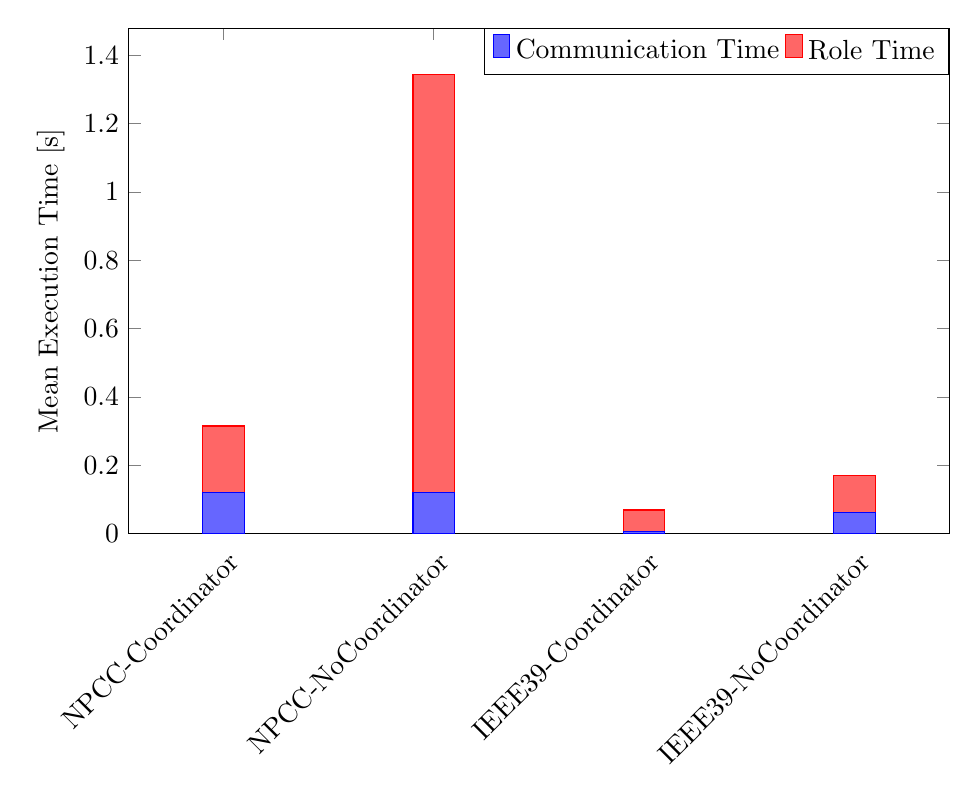
\begin{tikzpicture}
\begin{axis}[
    ybar stacked,
    bar width=15pt,
    width=12cm,
    height=8cm,
    ylabel={Mean Execution Time [s]},
    symbolic x coords={
        NPCC-Coordinator, NPCC-NoCoordinator, IEEE39-Coordinator, IEEE39-NoCoordinator
    },
    xtick=data,
    x tick label style={rotate=45, anchor=east, yshift=-0.3cm},
    ymin=0,
    enlarge x limits=0.15,
    legend style={
        at={(1,1)}, anchor=north east, legend columns=2
    }
]

% Example data (replace with your own)
\addplot+[fill=blue!60] coordinates {
    (NPCC-Coordinator, 0.121)
    (IEEE39-Coordinator, 0.0052)
    (NPCC-NoCoordinator,  0.121)
    (IEEE39-NoCoordinator, 0.061)
};

\addplot+[fill=red!60] coordinates {
    (NPCC-Coordinator, 0.194)
    (IEEE39-Coordinator, 0.064)
    (NPCC-NoCoordinator, 1.2237)
    (IEEE39-NoCoordinator, 0.11)
};

\legend{Communication Time, Role Time}

\end{axis}
\end{tikzpicture}
\caption{Mean execution time per iteration of MPC for NPCC and IEEE39 Comparison.}
\label{fig:meantime}
\end{figure}

Overall, we observe in \ref{fig:meantime} that the deployment with the coordinating role scales and performs better in both cases. The difference for the NPCC case is particularly significant, with a tenfold improvement for the centralized scheme. This can be due to very different factors but one possible explanation is that having exclusives roles for the coordination is more efficient than using a single one running in a single agent. However, the centralized scheme also presented issues during testing, as it occasionally exceeded COLMENA's capacity to handle data, which could result in crashes. Even in normal operations we could also risk certain loss of data during the exchanges. In this sense the decentralized scheme looks more robust. 

\subsection*{Test 3: Role Scalability}

In this section we run the same setup but we deploy previous roles with their respective KPIs and see how they all respond to the perturbation in the grid. For this case we also scale back the number of areas controlled by a MPC agent because the COLMENA testing was not able to handle the amount of data produced by so many agents. Overall we deploy the following agents. The objective of this test is to see multiple roles being activated when the KPI are broken and changing the grid to restore the KPI (the frequency) to its desired value.

\begin{itemize}
\item 3 agents with \texttt{AREA} requirement
\item 3 agents with \texttt{GENERATOR} requirement
\item 1 agent with \texttt{CONVERTER} requirement
\end{itemize}

We also slightly change the KPIs for a better frequency response. Instead of having the same KPI related to the frequency the MPC role will be activated when $\omega \leq 1.001$ while the automatic frequency control role will only be activated when $1.0001 \leq \omega \leq 1.001$. This change makes it so that the different roles don't interfere with each other and they both have more clear goals. The MPC control is used when the frequency deviation is greater while the automatic frequency control is activated for tunning the frequency in a finner way. Finally, the Grid Forming Role is activated also when $\omega \leq 1.001$  and the monitoring role has no KPI and monitors the frequency in the specific generator paired agents. To run this test you just need to change the change the \texttt{script\_name} variable when calling the script \texttt{colmena\_mpc.py} and call it adding \texttt{script\_name = mpc\_with\_multiple\_roles\_kpi} and also setting the attribute \texttt{converter = True} in \texttt{config.py}. 

We perform 2 test in 2 different grids, one with a controllable converter and one without. The first test makes us able to see how the automatic grid control affects the response \ref{fig:test_pid}. In the second one we add a converter to grid initially in grid following mode that is responsible for the small initial oscillations in the grid at the beginning of the simulation.

\begin{figure}[ht]
\centering
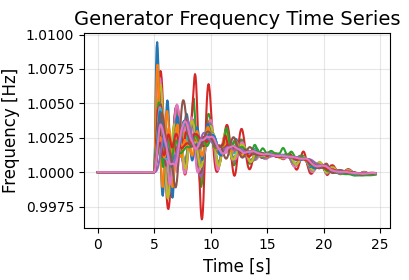
\includegraphics[width=0.8\textwidth]{figures/npcc_pid.png} % Replace with your actual image file path
\caption{Frequency timeseries of generators in test 3.}
\label{fig:test_pid}
\end{figure}


\begin{figure}[ht]
\centering
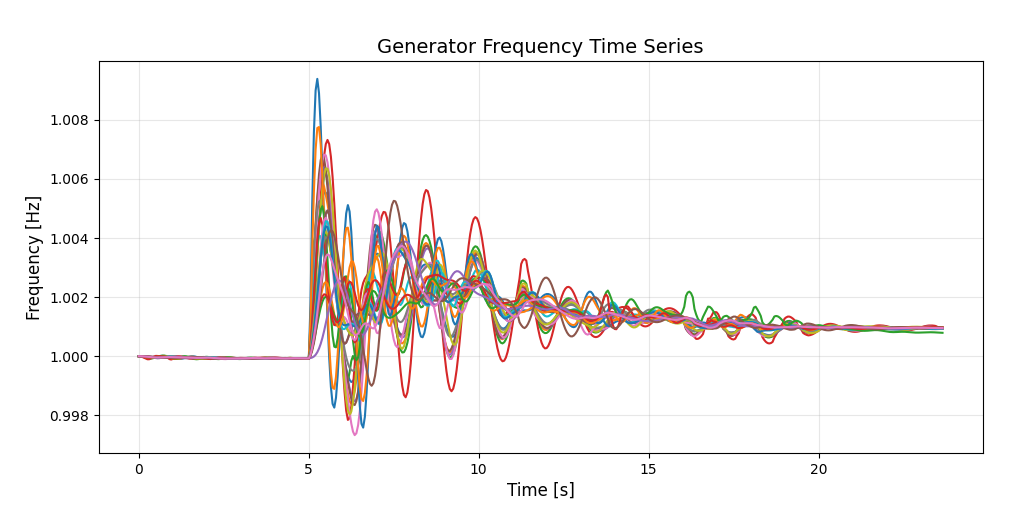
\includegraphics[width=0.8\textwidth]{figures/npcc_gfm.png} % Replace with your actual image file path
\caption{Frequency timeseries of generators in test with converters.}
\label{fig:test_gfm}
\end{figure}

 Overall, we see how the different roles manage to control the frequency \ref{fig:test_pid},\ref{fig:test_gfm} althought the effect of the automatic control role is noticable while the GFM role effect is less visible. The change of mode in the converter is properly simulated by ANDES and its voltage and  values that are within the admissible range. We also observe that the rest of the devices of the grid also behave in a desirable manner: the voltages of the buses are also within an acceptable range \ref{fig:bus_v} and the grid simulation is responds well to the actions of the different agents. In the case of the converter, voltage and frequency are also close to the pre perturbation value, the jump close the 6 second mark is due to the GFM role being activated, the resulting voltage being more stable than other the voltage in other buses. 

\begin{figure}[ht]
\centering
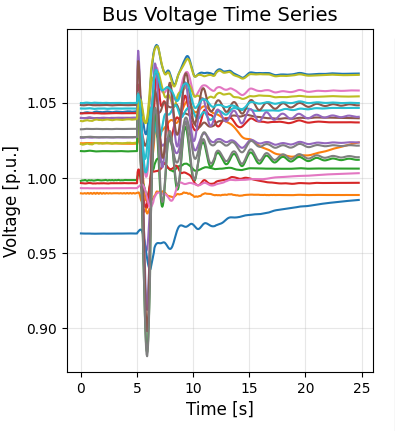
\includegraphics[width=0.8\textwidth]{figures/bus_voltage.png} % Replace with your actual image file path
\caption{Sample of bus voltages time series.}
\label{fig:bus_v}
\end{figure}

\begin{figure}[ht]
\centering
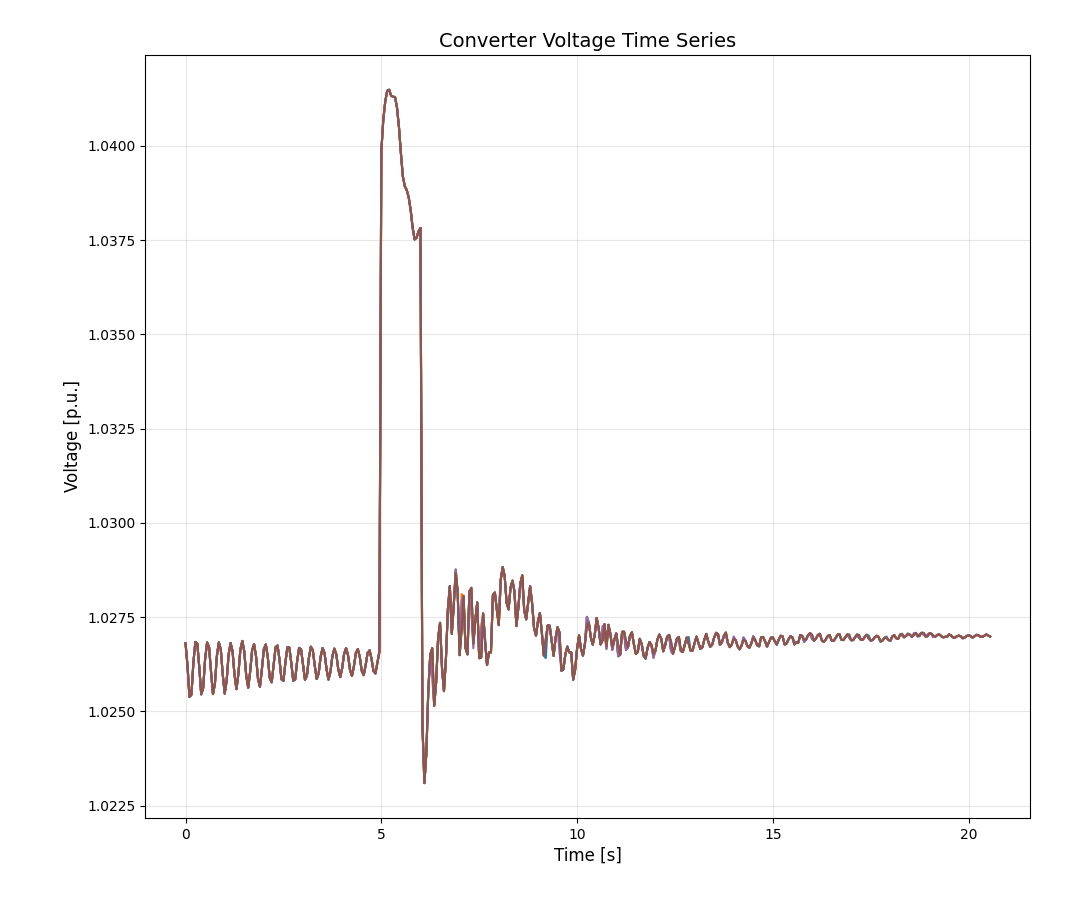
\includegraphics[width=0.8\textwidth]{figures/converter.png} % Replace with your actual image file path
\caption{Converter voltage time series .}
\label{fig:bus_v}
\end{figure}

\section{Milestones - COLMENA Evaluation}

\subsection*{Milestone 1: Testing of component behavior}

The completion of this milestone is demonstrated through an evaluation of the entire COLMENA prototype, including the integration and deployment of various roles within the Andes platform. The prototype was subjected to an extensive range of conventional and abnormal operating scenarios, where different agents and roles were tested for their ability to work cohesively and respond to disturbances in the grid. Each role, from the coordinator to the various agent types managing power flows, generation, and converters, were evaluated using the test suite specified earlier. In the end, all the different components worked properly to simulate a grid where the different roles can change the grid dynamically by acting on different electrical devices such as generators and converters.

\subsection*{Milestone 2: Measurement and evaluation of performance indicators}

Milestone 2 was achieved by conducting a study of key performance indicators (KPIs) for the COLMENA prototype. A series of tests were carried out to measure network robustness, voltage ranges, device behavior and computational time across different configurations of the initial system. These KPIs were assessed under a variety of operating scenarios, specifically during frequency increases due a loss of loads. The results demonstrated that the system was able to adapt effectively to changes, with quick reconfigurations of the grid to adapt to disturbances. The use of edge computing allowed for rapid decision-making, which contributed to the short recovery times observed during tests. The system showed the capacity to maintain voltage and frequency stability. These findings confirm that the COLMENA platform is capable of handling dynamic conditions and can reconfigure the grid within a short time frame. Additionally, the test results highlighted areas where the algorithms could be optimized further, providing valuable insights for future improvements.

\newpage
\clearpage
\nocite{*}  
\printbibliography
\end{document}
